\subsection{Постановка задачи}
3.4. Вычислить первую и вторую производную от таблично заданной функции $y_i = f(x_i), i = 0,1,2,3,4$ в точке $x= X^*$.  

{\bfseries Вариант:} 19
    \begin{equation}
		X^*=0.1
    \end{equation}
    \begin{center}
        \begin{tabular}{ |c|c|c|c|c|c| } 
			 \hline
			 $i$ & 0 & 1 & 2 & 3 & 4 \\ 
			 \hline
			 $x_i$ & -1 & 0 & 1 & 2 & 3 \\ 
			 \hline
			 $f_i$ & -1.7854 & 0.0 & 1.7854 & 3.1071 & 4.249 \\ 
			 \hline
        \end{tabular}
    \end{center}
\pagebreak

\subsection{Результаты работы}
\begin{figure}[h!]
\centering
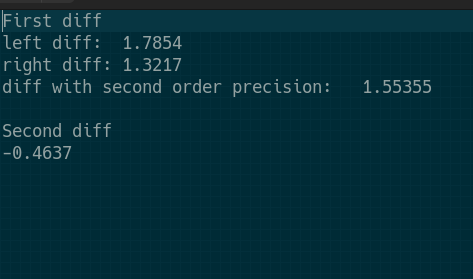
\includegraphics[width=.5\textwidth]{lab3.4}
\caption{Вывод в консоли}
\end{figure}


\subsection{Исходный код}
\lstinputlisting[title=\texttt{Lab3.4.cpp}]{../stud/saifullin/task3.4/Lab3.4.cpp}
\pagebreak

